\section{Introducción}

\IEEEPARstart{D}{iferentes} alternativas energéticas han sido ampliamente exploradas en la
 literatura.
 En particular, la energía eólica ha registrado una importante acogida,
 en especial en Europa donde en las últimas décadas se puede evidenciar
 un crecimiento promedio anual de hasta el 30\% \cite{ewea2004windindustry}.
 Sin embargo, la implementación de una solución eólica no resulta trivial.
 La primera etapa a afrontar es la ubicación de potenciales lugares donde
 las condiciones de viento resulten apropiadas.
 En este sentido, las principales características a monitorear son las velocidad
 y dirección del viento y se espera poder ubicar geográficamente aquellos
 lugares donde estas características registren elevados promedios durante
 un periodo considerable de tiempo. El proyecto general ``Análisis de oportunidades
 energéticas con fuentes alternativas para el departame
nto de Nariño'' tiene como uno de sus objetivos cumplir con este propósito.

A través de un proveedor externo se tiene acceso a series de tiempo de los
 últimos diez años con información sobre la ubicación de la muestra (latitud
 y longitud) y la correspondiente velocidad y orientación del viento.
 Con esta base de datos resultaría sencillo generar mapas del potencial
 eólico para el departamento.
 Sin embargo, también resulta de gran importancia para el proyecto conducir
 investigación de alto nivel orientada al análisis de los datos generados
 y disponibles.
 Esta investigación busca analizar las fuentes de datos disponibles en procura
 de la extracción de patrones secuenciales en el comportamiento de la dirección
 y velocidad del viento en aquellos lugares con potencial eólico.
 Dichos patrones servirán de soporte para la detección de anomalías y para
 la toma de decisiones a la hora de la implementación de una solución final.
 
 El area de estudio de esta investigación fue el departamento de Nariño (Colombia)
el cual esta ubicado en el extremo sur occidental de Colombia, en la frontera con 
Ecuador con una extensión aproximada de 33.268 km, una población de 1,702 millones según
el censo de 2013, su ubicación 
esta en latitud 00° 31' 08'' y 02° 41' 08'' Norte, Longitud 76° 51' 19'' y 79° 01' 34'' Oeste.

\begin{figure}
  \centering
  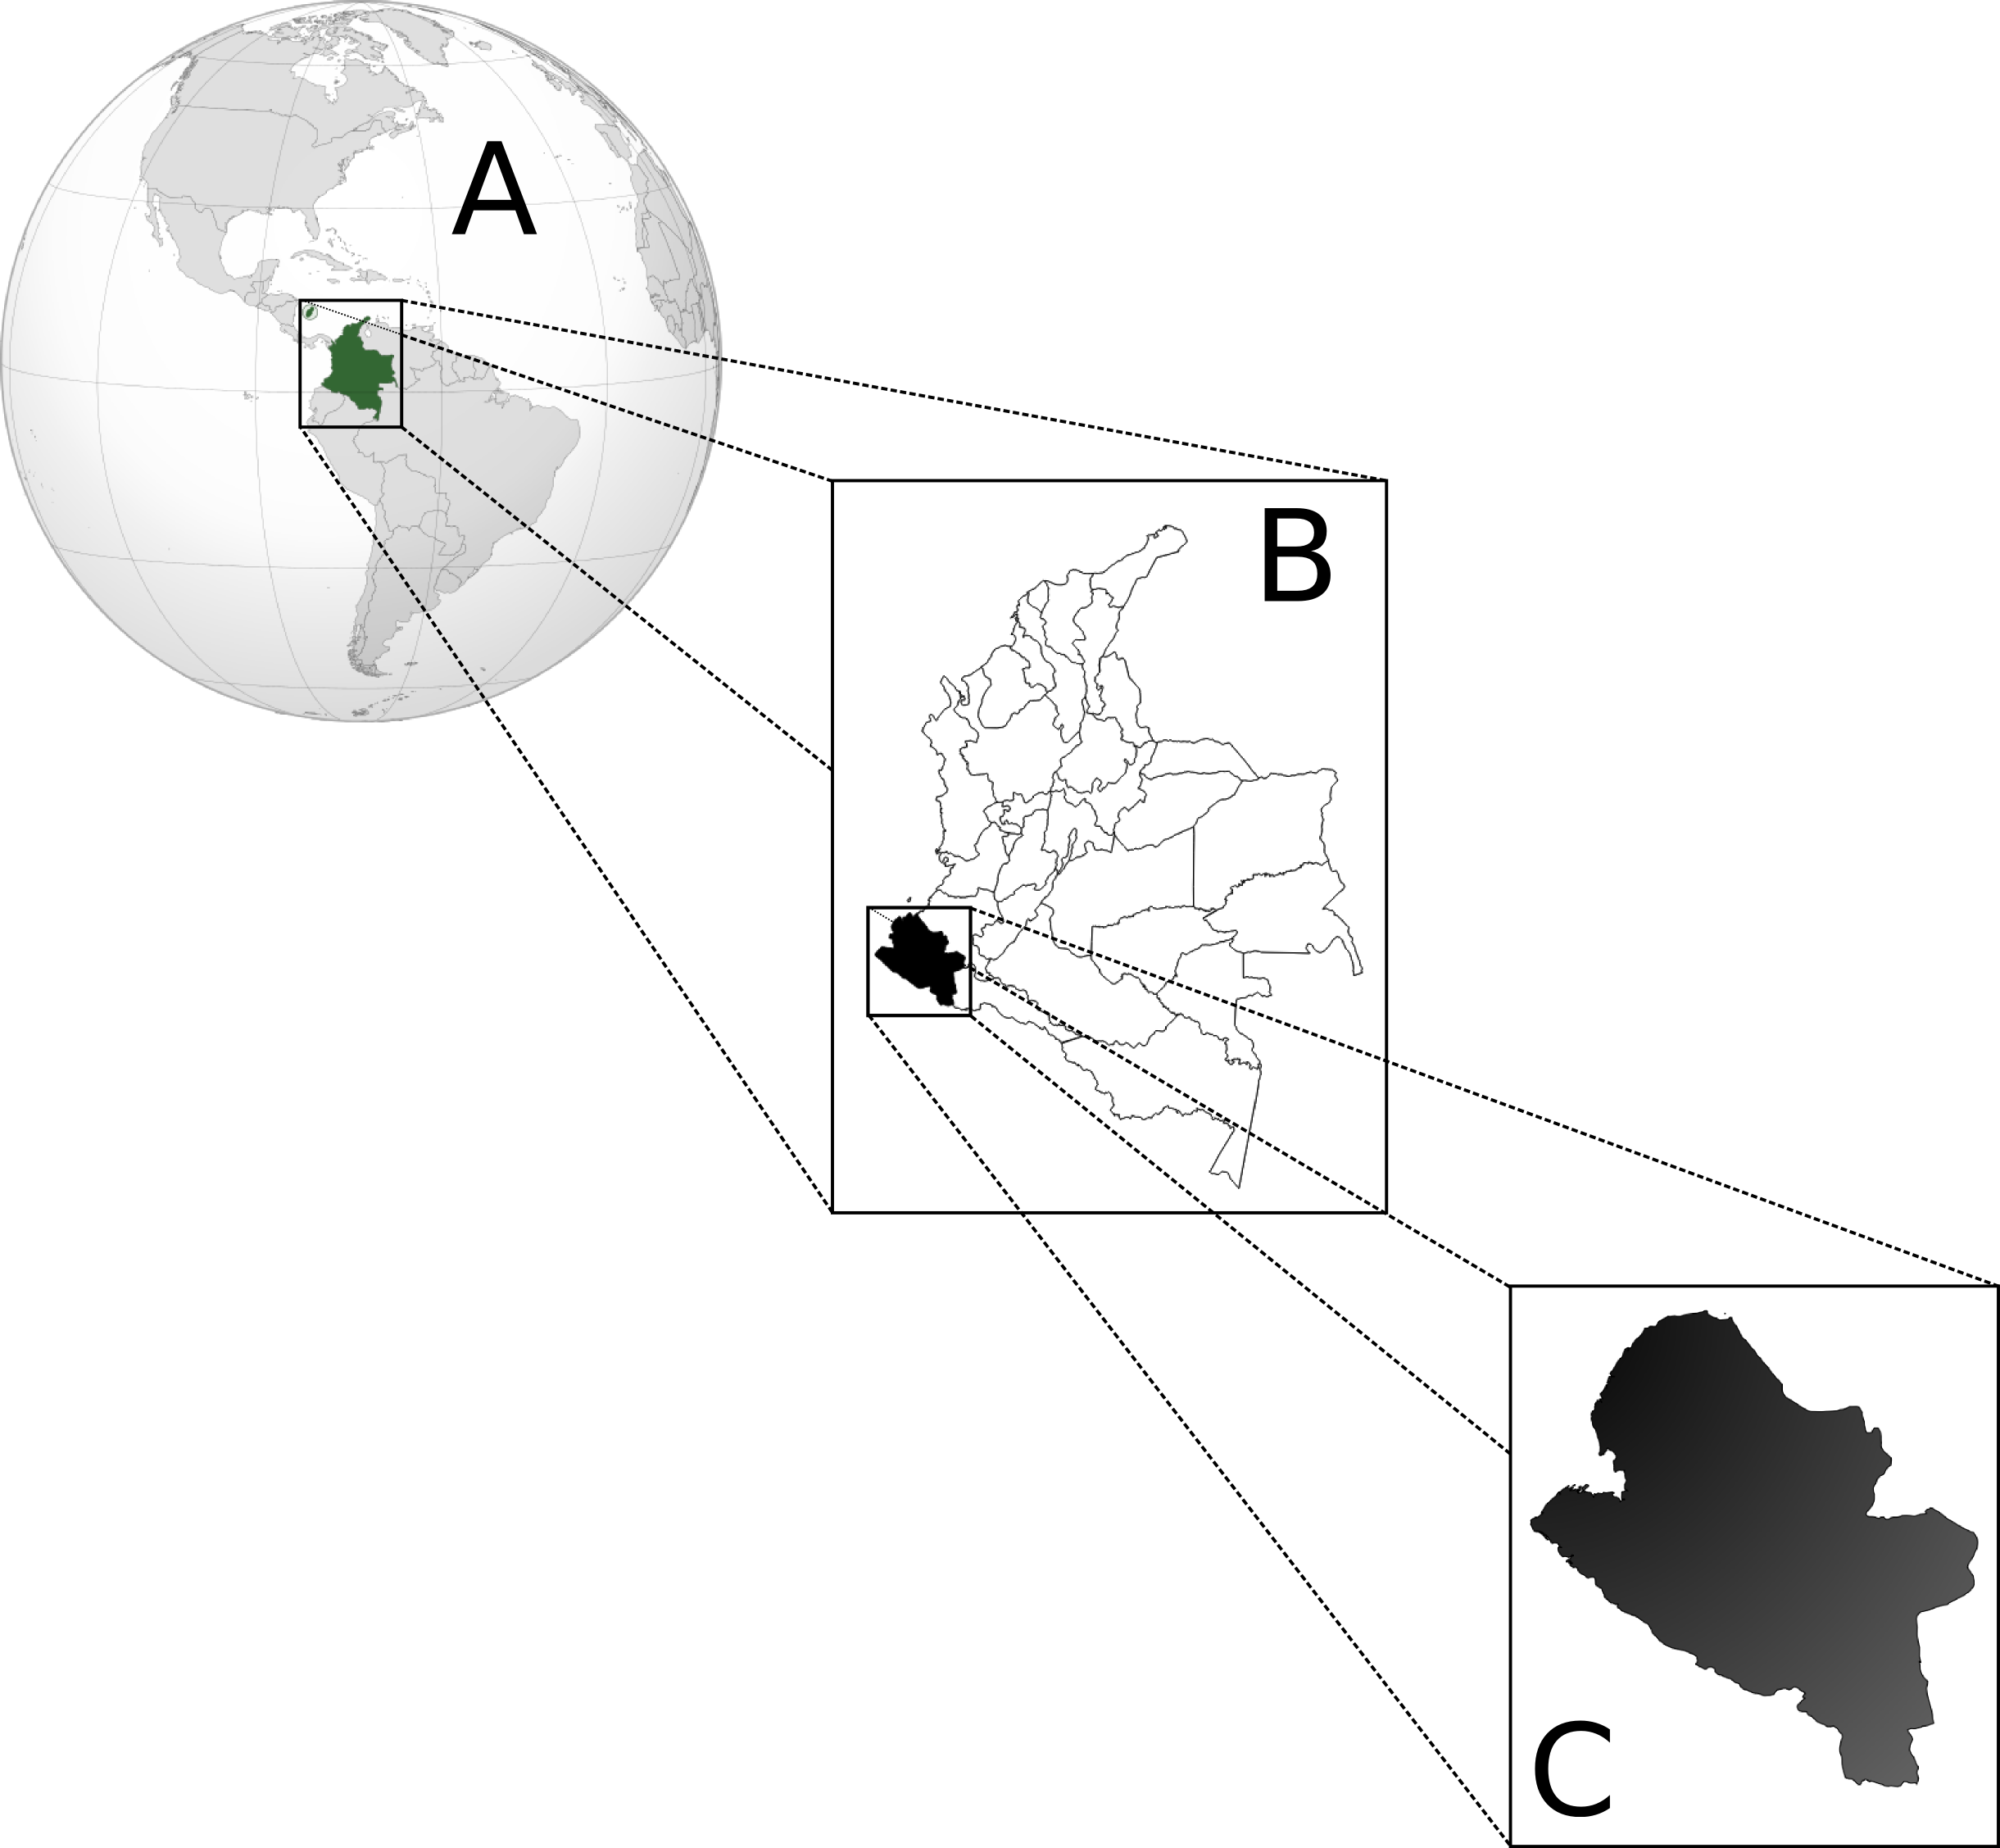
\includegraphics[width = 8cm]{locationNarino.png}
  \caption{Localización area de estudio}
  \label{fig:locationNarino}
\end{figure}